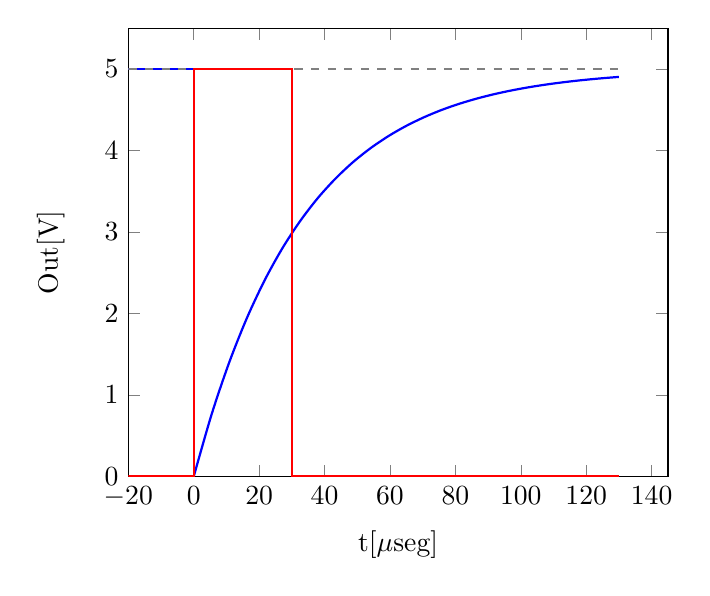
\begin{tikzpicture}
 \begin{axis}[
   scaled ticks=false,
   xmin=-20,
   ymin=0,
    x label style={at={(axis description cs:0.5,-0.1)},anchor=north},
    y label style={at={(axis description cs:-0.1,.5)},rotate=0,anchor=south},
    xlabel={t[$\mu$seg]},
    ylabel={Out[V]}
   ]
    \addplot[domain=0:130, blue, thick,smooth] {5*(1-e^(-x/33))};
    \addplot[domain=-20:100, const plot, blue, no marks, thick] coordinates {(-20,5) (0,5) (0,0)};
    \addplot[domain=-20:130, gray, dashed] {5};
    \addplot[domain=-20:100, const plot, red, no marks, thick] coordinates {(-20,0) (0,0) (0,5) (30,5) (30,0) (130,0)};
\end{axis}
\end{tikzpicture}
